For this section see: Multiple View Geometry in Computer Vision.

\subsection{Pinhole camera model}

Mathematically, a \textbf{camera} is just a mapping from $\mathbb{R}^3$ to $\mathbb{R}^2$. A \textbf{camera model} is then a linear transformation represented by a matrix with particular properties that represent the camera under study. 

The pinhole camera model describes the mathematical relationship between the coordinates of a 3D point and its projection onto the image plane of an ideal pinhole camera, where the camera aperture is described as a point and no lenses are used to focus light.

\begin{figure}[H]
\centering
\makebox[\textwidth][c]{
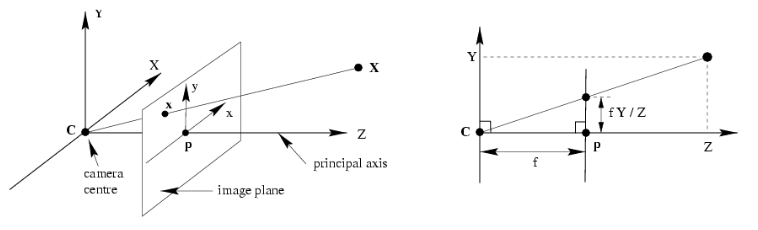
\includegraphics[scale=0.75]{./images/pinhole.png}
}
\end{figure}

\subsection{Notions of projective geometry}

It is better to express this equations in terms of projective geometry concepts as the mappings of this setting (projectivities) are more general and have good property-preserving characteristics.

If we recall (from a book in projective geometry) that the projective plane can be understood as the three dimensional vector lines (with origin in the camera centre) and state that a projection is a linear map in the three dimensional space, then the following properties are obvious:

\begin{itemize}
\item Points are mapped to points but projection of points on focal plane is undefined.
\item Lines are mapped to lines but the line through focal point projects to a point (an infinite point).
\item Planes are mapped to planes but the plane through focal point projects to line (the infinite line).
\end{itemize}

In particular, a projection preserves collinearity.

Passing from 3D to 2D implies a lost of information. For instance we loose angles and distances since projections are not isometries. In some occasions, some information may be recovered using multiple images, details of the camera or simply knowing the size of the represented objects.

A good property of projective geometry is that any two lines intersect at infinity. So we can say that each "direction" in space has its own vanishing point meaning that all lines in that direction converge at that point. Again, directions parallel to the image plane don't appear to have a vanishing point although in formal geometry this point is a point at infinity. It is also clear that all directions in the same plane have vanishing points on the same line.

In projective geometry we can interchange the notion of concurrent lines and collinear points. This is known as \textbf{duality}. Therefore if we state that any two lines intersect at a point (with parallel lines intersecting at some point of the infinite line) we can state that any two points determine a unique line.

It is time to make a classification of the type of mappings that we have encountered this course:

\begin{itemize}
\item Isometries or Euclidian tranformations: rotations and translations they preserve metric notions like angles, surfaces and lengths. 
\item Similarities: they are compositions of isometries and homotheties. They preserve angles and length proportions. 
\item Affine transforms: they are bijective applications in the plane. They preserve parallelism, length proportions and surface proportions. (6 degrees of freedom)
\item Projectivities transforms: they are bijective applications in the plane. They preserve collinearity. (8 degrees of freedom)
\end{itemize}

\subsection{Uses of homography}
\begin{itemize}
\item If we look at the equation of the camera projection matrix, we will see that it has parameters that depend on the camera settings (called intrinsic parameters) and some parameters to perform the euclidean transformation from the world coordinate system to the camera coordinate system (extrinsic parameters).
It is necessary to estimate these parameters. A way to do so is to relate them with homographies.

\begin{figure}[H]
\centering
\makebox[\textwidth][c]{
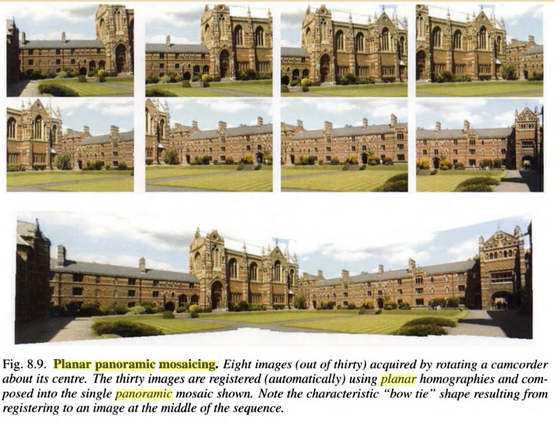
\includegraphics[scale=0.75]{./images/mosaic.png}
}
\end{figure}

\item Another use is forming \textbf{mosaics of images} like the one above, the principles to form this images is performing an homography between pairs of images as show below:


\begin{figure}[H]
\centering
\makebox[\textwidth][c]{
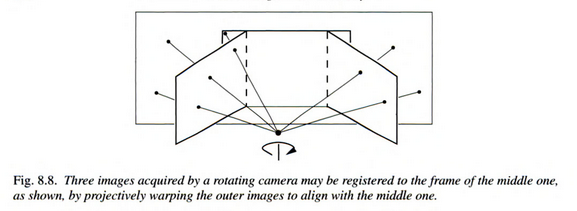
\includegraphics[scale=0.55]{./images/principle.png}
}
\end{figure}


\item They can be also used for \textbf{rendering textures} by applying homographies between planar scene surfaces and image planes.

\item In photography and cinematography, perspective distortion is a warping or transformation of an object and its surrounding area that differs significantly from what the object would look like with a normal focal length, due to the relative scale of nearby and distant features. Perspective distortion is determined by the relative distances at which the image is captured and viewed, and is due to the angle of view of the image (as captured) being either wider or narrower than the angle of view at which the image is viewed, hence the apparent relative distances differing from what is expected. 

Perspective distortion can be reduced using homographies.


\begin{figure}[H]
\centering
\makebox[\textwidth][c]{
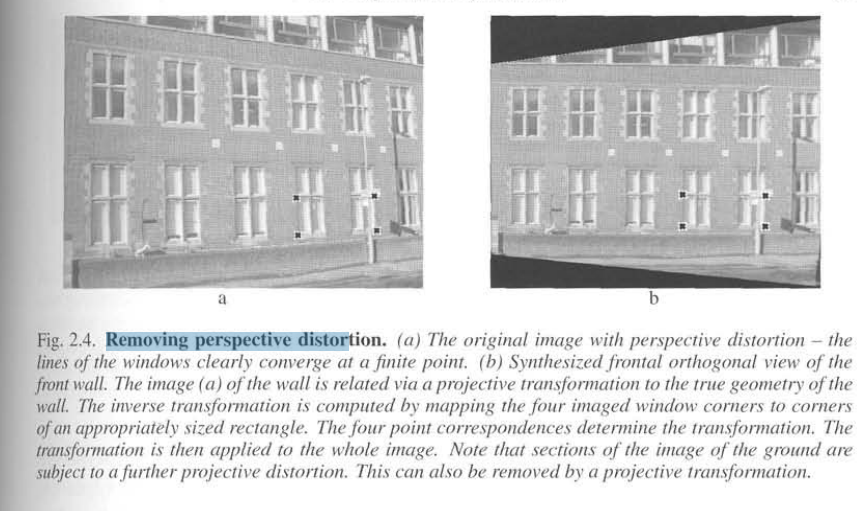
\includegraphics[scale=0.55]{./images/distort.png}
}
\end{figure}

\end{itemize}








